% Тут используется класс, установленный на сервере Papeeria. На случай, если
% текст понадобится редактировать где-то в другом месте, рядом лежит файл matmex-diploma-custom.cls
% который в момент своего создания был идентичен классу, установленному на сервере.
% Для того, чтобы им воспользоваться, замените matmex-diploma на matmex-diploma-custom
% Если вы работаете исключительно в Papeeria то мы настоятельно рекомендуем пользоваться
% классом matmex-diploma, поскольку он будет автоматически обновляться по мере внесения корректив
%

% По умолчанию используется шрифт 14 размера. Если нужен 12-й шрифт, уберите опцию [14pt]
%\documentclass[14pt]{matmex-diploma-custom}
\documentclass[14pt]{matmex-diploma}
\usepackage{multirow}
\usepackage{multirow}
\usepackage[table,xcdraw]{xcolor}
\usepackage{graphicx}
\usepackage{subcaption}
\usepackage{lscape}
\usepackage{longtable}
\usepackage{tikz}

\begin{document}
% Год, город, название университета и факультета предопределены,
% но можно и поменять.
% Если англоязычная титульная страница не нужна, то ее можно просто удалить.
\filltitle{ru}{
    chair              = {Программная инженерия\\ Кафедра системного программирования},
    title              = {Разработка библиотеки для визуализации 3D графики},
    % Здесь указывается тип работы. Возможные значения:
    %   coursework - Курсовая работа
    %   diploma - Диплом специалиста
    %   master - Диплом магистра
    %   bachelor - Диплом бакалавра
    type               = {coursework},
    position           = {студента},
    group              = 371,
    author             = {Орачев Егор Станиславович},
    supervisorPosition = {ст. преп.},
    supervisor         = {А. А. Пименов},
    % reviewerPosition   = {ст. преп.},
    % reviewer           = {Привалов А.\,И.},
    % chairHeadPosition  = {д.\,ф.-м.\,н., профессор},
    % chairHead          = {Хунта К.\,Х.},
    university         = {Санкт-Петербургский Государственный Университет},
    % faculty            = {Математико-механический факультет},
    city               = {Санкт-Петербург},
    year               = {2020}
}

% \filltitle{en}{
%     chair              = {The Meaning of Life \\ Uselessness of Everything},
%     title              = {Empty subset as closed set},
%     author             = {Edelweis Mashkin},
%     supervisorPosition = {professor},
%     supervisor         = {Amvrosy Vibegallo},
%     reviewerPosition   = {assistant},
%     reviewer           = {Alexander Privalov},
%     chairHeadPosition  = {professor},
%     chairHead          = {Christobal Junta},
% }

\maketitle
\tableofcontents

% ---------------------------------------------------------------------------- %

\section*{Введение}

Трехмерная графика --- раздел компьютерной графики, посвященный методам визуализации объемных моделей и объектов, описанных в 3D (3-dimensional) пространстве. К основным областям применения трехмерной графики можно отнести: системы автоматизированного проектирования, кинематограф, анимацию, видеоигры, симуляторы и многое другое.

Существует несколько способов построения изображения по трехмерным данным, одними из которых являются: растеризация примитивов, трассировка лучей, трассировка пути. Применение конкретного способа с последующей его конфигурацией обуславливается различными факторами:

\begin{itemize}
    \item Временными ресурсами. При работе в режиме реального времени максимальный интервал генерации изображения составляет приблизительно 33 миллисекунды (соответствует частоте обновления 30 Гц), что позволяет создать непрерывный для человеческого глаза видеопоток.
    \item Вычислительными ресурсами, предоставляемыми конкретной платформой, вместе со спецификой их использования. К примеру, мобильные устройства накладывают существенные ограничения на энергопотребление и не имеют активное охлаждение.
    \item Объемом отображаемых данных.
    \item Качеством отображения, которое может характеризоваться как фото-реалистичное, физически корректное, кинематографичное, "мультяшное"~\cite{wiki:celshading} и так далее. 
\end{itemize}

Наличие вышеизложенных факторов в сочетании с многочисленными требованиями реальных проектов, связанных с визуализацией данных, создает ряд проблем при поиске уже готовых графических решений и при их непосредственной интеграции в систему.       

В проекте CoreCVS~\cite{github:corecvs} (Computer Vision Primitives Library) в рамках работы над библиотекой для симуляции физики полетов дронов разработчики столкнулись с необходимость визуализации процесса симуляции как для отладки программ, так и для лучшего понимания того, как взаимодействуют объекты между собой. Для решения этой проблемы используется существующая в рамках проекта графическая библиотека, написанная с использованием OpenGL~\cite{spec:opengl} (Open Graphics Library), которая позволяет отображать относительно простую геометрию с базовой моделью освещения. Однако данная библиотека использует в своей основе уже устаревшее подмножество функциональности OpenGL, что создает необходимость значительного рефакторинга для дальнейшего ее использования.    

В итоге было принято решение разработать с нуля новую графическую библиотеку в рамках CoreCVS, которая не только бы замещала функциональность своей предшественницы, но и расширяла ее в соответствии с задачами, решаемыми как в текущих, так и в будущих проектах.

Данное решение мотивированно не только стремлением минимизировать количество сторонних зависимостей всего проекта, но и желанием использовать в качестве основы новейшее Vulkan API~\cite{spec:vulkan} (Vulkan Application Programming Interface), которое призвано заменить OpenGL в силу его морального устаревания. Анализ существующих решений также показал невозможность интеграции сторонних библиотек ввиду ряда причин, изложенных далее в тексте работы. 

\section{Постановка задачи}

Цель данной работы --- реализация библиотеки для визуализации трехмерной графики в реальном масштабе времени с возможностью использовать как низкоуровневый интерфейс для создания специфичных моделей отображения, так и высокоуровневые абстракции, предоставляющие стандартный способ визуализации объектов. Для ее достижения были выделены следующие задачи:

\begin{itemize}
    \item Исследование предметной области. Сравнение существующих решений
    \item Разработка и формализация требований к проекту
    \item Реализация компонентов графической библиотеки с учетом заявленных требований
    \item Реализация поддержки Vulkan API
\end{itemize}

% ---------------------------------------------------------------------------- %

\section{Терминология}

\begin{itemize}
    \item Графическая подсистема (англ. Graphical backend) --- модуль программы, реализующий графическую функциональность приложения.
    \item Шейдер (ангд. Shader) --- программа, предназначенная для исполнения на графическом процессоре.
    \item Материал --- контейнер, которых хранит описание поверхности объекта в виде набора атрибутов и некоторую программу, которая контролирует процесс обработки данного материала.
    \item Графический интерфейс (англ. Graphical API) --- интерфейс для взаимодействия с графическим ускорителем системы.
    \item Application Programming Interface (API) --- интерфейс прикладного программирования.
    \item Central Processing Unit (CPU) --- центральный процессор.
    \item Graphical Processing Unit (GPU) --- графический процессор.
    \item Graphical User Interface (GUI) --- графический пользовательский интерфейс.
\end{itemize}

% ---------------------------------------------------------------------------- %

\section{Требования к проекту}

Основные функциональные требования, которые вытекают прежде всего из задач, решаемых в рамках проекта CoreCVS, изложены далее:

\begin{itemize}
    \item Генерация изображения в режиме реального времени: в своей основе библиотека полагается на алгоритм растеризации геометрии с использованием \textit{Z-буфера}~\cite{realtimerendering}, что позволяет при должном количестве геометрии и вычислительных ресурсах генерировать изображения с частотой, достаточной для создания псевдонепрерывного видеопотока.
    \item Кроссплатформенность: библиотека компилируется и работает на линейке основных операционных систем (Window, Linux, MacOS).
    \item Независимость от графического интерфейса: библиотека взаимодействует с видеоускорителем системы через унифицированный интерфейс, который сам по себе является частью проекта.
    \item Поддержка Vulkan: доступ к данному API осуществляется через интерфейс, представленный в предыдущем пункте. 
    \item Независимость от структуры сцены: библиотека поддерживает список видимых объектов и осуществляет их последовательное отображение. Иерархию сцены, зависимости между объектами определят пользователь. 
    \item Система материалов: материалы предоставляют типобезопасный интерфейс для конфигурации параметров отображения на GPU. 
    \item Система хранения геометрии: возможность создавать и использовать геометрические объекты с произвольным набором атрибутов. 
    \item Независимость от оконной системы: финальное изображение выводиться на экран, в виджет GUI системы, либо сохраняется во внеэкранном буфере.
\end{itemize}

% ---------------------------------------------------------------------------- %

\section{Существующие решения}
    
В данном разделе проводится обзор и сравнение существующих графических решений с открытым исходным кодом, доступным для свободного использования. Критерии обзора вытекают прежде всего из требований, изложенных ранее. Основные факторы для включения в рассмотрение: наличие документации и обучающих материалов, активная поддержка или разработка, интеграция с Vulkan, поддержка широкого класса графических интерфейсов, индексация\footnote{Дата обращения: 11.12.2019} на хостинге GitHub.

\subsection{BSF}

BSF (bs framework) --- кросс-платформенная С++14 библиотека, разрабатываемая Game Foundry \cite{github:bsf}. Предоставляет унифицированную базу для разработки графических приложений реального времени, видеоигр и инструментов программирования. Поддерживаемые графические интерфейсы: Vulkan, OpenGL, DirectX. Функциональность: конвейер экранных пост-эффектов, отложенное, физически корректное затенение, каскадная генерация теней, система материалов.

\subsection{Ogre3D}

Ogre3D (Object-Oriented Graphics Rendering Engine) --- кросс-платформенная С++ графическая библиотека, разрабатываемая открытым сообществом~\cite{github:ogre3d}. В качестве графических интерфейсов поддерживает OpenGL, DirectX, WebGL. Функциональность: система материалов и пост-эффектов, менеджмент ресурсов, система анимации, граф сцены.  

\subsection{Filament}
    
Filament --- кросс-платформенная С++ библиотека графики, неофициально поддерживаемая Google~\cite{github:filament} и открытым сообществом разработчиков. Спроектирована таким образом, чтобы быть максимально компактной и эффективной для Android платформы. Поддерживает OpenGL, Vulkan API, WebGL. Предоставляет С++, Java, JavaScript интерфейсы. Основные графические возможности: физически корректное затенение, освещение на основе изображения, система материалов, камера с имитацией физических параметров параметрами, базовые пост-эффекты. 

\subsection{Концептуальные недостатки}

Несмотря на многочисленную функциональность, которой обладают рассмотренные решения, они не в полной мере удовлетворяют требованиям проекта CoreCVS. В частности, BFS и Ogre3D прежде всего ориентированны на разработку видео игр, поэтому данные библиотеки сильно зависят как от иерархической структуры сцены, так и от обработки данных. Они предоставляют собственные форматы геометрии, языки описания шейдеров и методы загрузки ресурсов, таких как модели, текстуры. Данная функциональность избыточна, так как в проекте CoreCVS уже существуют модули по обработке 3D геометрии и изображений. 

\begin{figure}[h]
     \caption{Сравнение существующих решений по основным критериям}
     \centering
     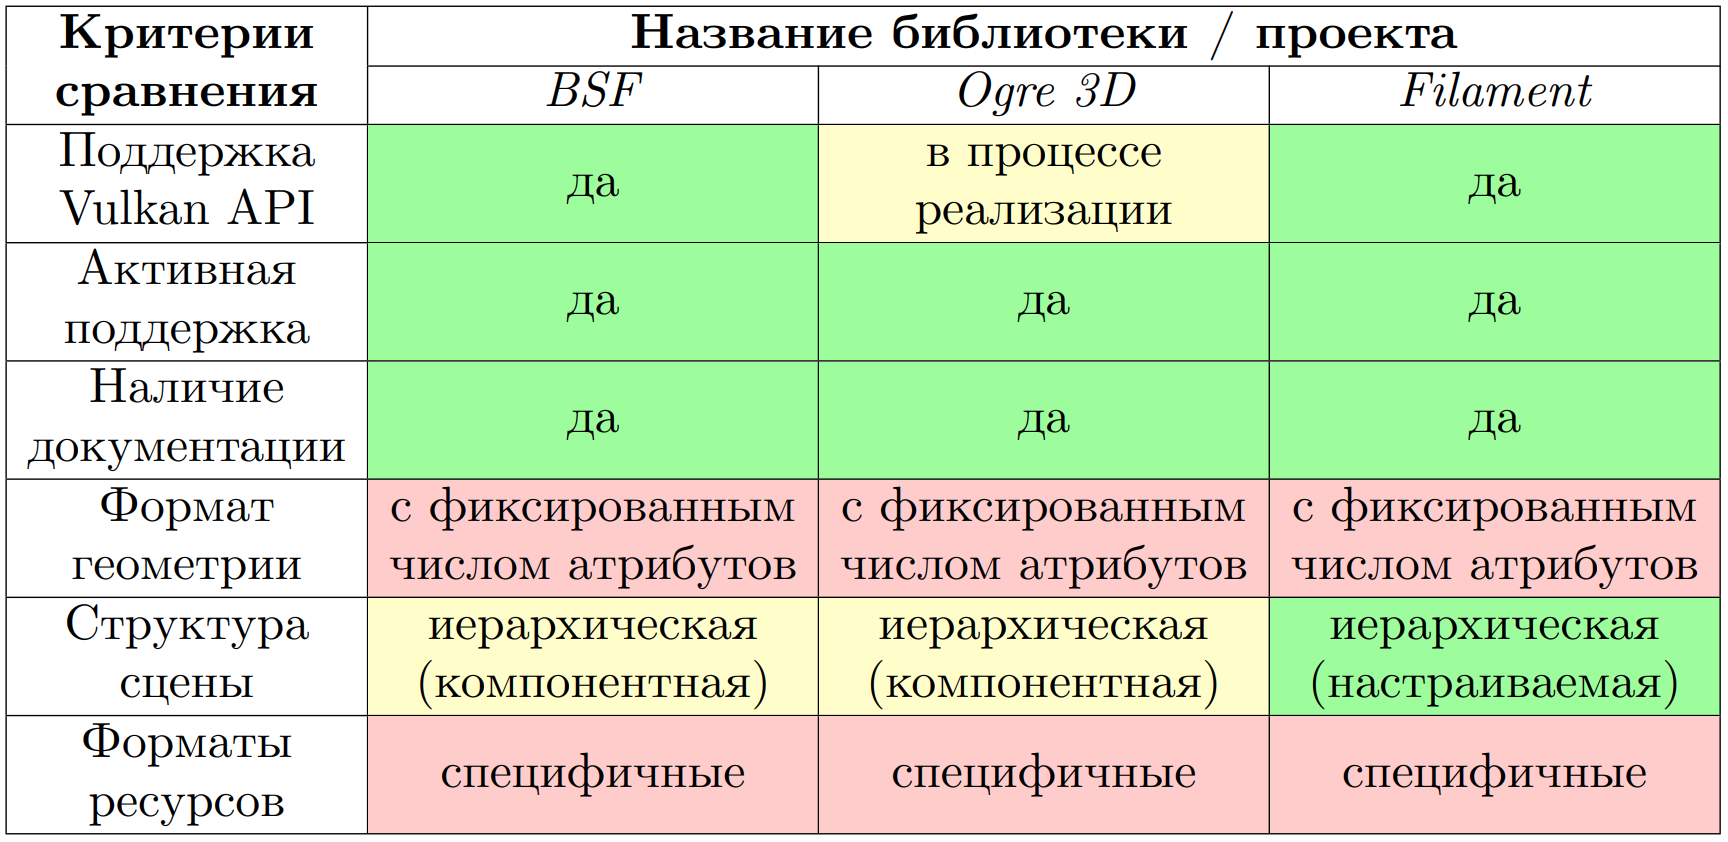
\includegraphics[width=1.0\textwidth]{pictures/Compare}
     \label{tab:compare:libs}
\end{figure}

Проект Filament имеет больший фокус на графическую составляющую, однако он в первую очередь ориентирован на создание физически корректного освещения на Android платформе, что выражается с существенно меньшей гибкости в настройке как самого освещения, так и экранных эффектов, создание которых практически ограничено на мобильных устройствах ввиду их высокой вычислительной сложности.

Детальное сравнение рассмотренных решений по основным критериям представлено на рис.~\ref{tab:compare:libs}. Красным цветом выделены критические аспекты, желтым --- устранимые, но нежелательные особенности, зеленым --- полностью приемлемые функциональные возможности.

Поэтому было принято решение отказаться от интеграции одного из существующих решений и сосредоточиться на разработке новой библиотеки, с учетом всей функциональности, которая в той или иной форме уже представлена в проекте CoreCVS. 

% ---------------------------------------------------------------------------- %

\section{Vulkan API}

Vulkan --- это кросс-платформенное API для работы с трехмерной графикой и параллельными вычислениями. Предоставляет C99 совместимый интерфейс для взаимодействия с GPU и спецификацию, которая описывает семантику исполнения программ. Впервые был представлен в феврале 2016 года. В настоящее время поддерживается консорциумом Khronos Group. 

\subsection{Обзор ключевых особенностей}

Vulkan является одним из представителей таких графических интерфейсов нового поколения, как Metal~\cite{spec:metal} и Direct3D~\cite{spec:direct3d}. В сравнении со стандартами прошлого поколения, Vulkan имеет ряд новых функциональных особенностей, которые призваны повысить эффективность работы конечных приложений:

\begin{itemize}
    \item Возможность работать на множестве операционных систем, включаю мобильную платформу.
    \item Меньшее количество ресурсов, используемых во время работы. Это достигается ручным управлением памятью, используемой драйвером как на CPU, так и на GPU, явным созданием и удалением графических конвейеров обработки примитивов.
    \item Лучшая расширяемость на платформах с несколькими ядрами. Драйвер позволяет формировать команды для GPU из нескольких потоков. 
    \item Универсальное представление GPU программ в бинарном формате SPIR-V~\cite{spec:spirv}. Это позволяет создавать шейдерные программы на любом из доступных языков, включая GLSL~\cite{spec:glsl} и HLSL~\cite{spec:hlsl}, и компилировать их в объектные модули независимо от конечной платформы. 
    \item Унифицированный менеджмент вычислительных ядер на GPU. Это позволяет использовать вычислительный конвейер посредством Vulkan API, не прибегая к сторонним вычислительным библиотекам, таким как Nvidia CUDA и OpenCL.
\end{itemize}

\subsection{Сравнение с другими графическими API}

В области разработки графических приложений существует ряд промышленных API, часть из которых уже была упомянута ранее в тексте работы. Direсt3D предоставляет схожую графическую функциональность, что и Vulkan, однако он доступен только на платформе от компании Microsoft. Графический API Metal, разрабатываемый корпорацией Apple, также доступен только на устройствах и системах этой компании. OpenGL является открытым стандартом, доступным на многих платформах, исключая мобильные устройства, где используется OpenGLES. Однако развитие данного API затруднено требования обратной совместимости, а поддержка его новых версий уже не осуществляется на некоторых устройствах\footnote{Компания Apple прекратила поддержку новых версий OpenGL в 2018, объявив официально данный API устаревшим на своей платформе}.       

Таким образом, было принято решение использовать Vulkan API в качестве основы для реализации данного проекта, так как он удовлетворяет функциональным требованиям разрабатываемой библиотеки и обладает активной поддержкой на основных платформах.

% ---------------------------------------------------------------------------- %

% \section{Текущий прогресс}

% Прогресс по проекту на данный момент:

% \begin{itemize}
%     \item Проведен обзор и сравнение существующих решений в соответствии с требованиям, предъявляемыми к разрабатываемой графической библиотеке. 
%     \item Проведен анализ существующих графических интерфейсов. Выбран Vulkan API как основа для реализации библиотеки по ряду причин, изложенных ранее в тексте работы.
%     \item Выбран стек технологий для реализации проекта (C++11, CMake, Vulkan SDK) с учетом функциональных требований и условий интеграции с библиотекой CoreCVS, в которой в качестве основного языка разработки используется C++11, а в качестве инструмента сборки и управления зависимостями используется CMake. 
%     \item Изучены обучающие материалы для работы с Vulkan SDK и официальная Vulkan API документация на уровне, необходимом для реализации проекта.
%     \item Настроен репозиторий проекта, система автоматической сборки библиотеки и запуска тестов, чтобы обеспечить работоспособность конечного решения на нескольких платформах.
%     \item На данный момент ведется активная работа над разработкой архитектуры системы и написанием необходимых модулей библиотеки.   
% \end{itemize}

% ---------------------------------------------------------------------------- %

\section{Описание реализации}

В данном разделе приводится описание общей структуры проекта и отдельных компонентов  графической библиотеки, реализация которых осуществлялась в рамках данной работы. Исходный код проекта опубликован на хостинге GitHub\footnote{Исходный код проекта: https://github.com/EgorOrachyov/Ignimbrite}. Работа по реализации библиотеки выполнялась совместно со студентом 371 группы Сультимом Цырендашиевым.

\subsection{Структура проекта}

Основные компоненты и классы разработанной графической библиотеки библиотеки представлены на рис.~\ref{fig:library:uml}. 

В качестве языка программирования для разработки использовался C++11, для управления процессом сборки и подключения сторонних зависимостей использовался CMake 3.14, что соответствует требованиям проекта и условиям интеграции с библиотекой CoreCVS.

Для поддержки сборки проекта для трех основных платформ была настроена непрерывная интеграция на платформе Github Actions.

\begin{figure}[]
     \caption{UML диаграмма основных компонентов и классов разработанной графической библиотеки}
     \centering
     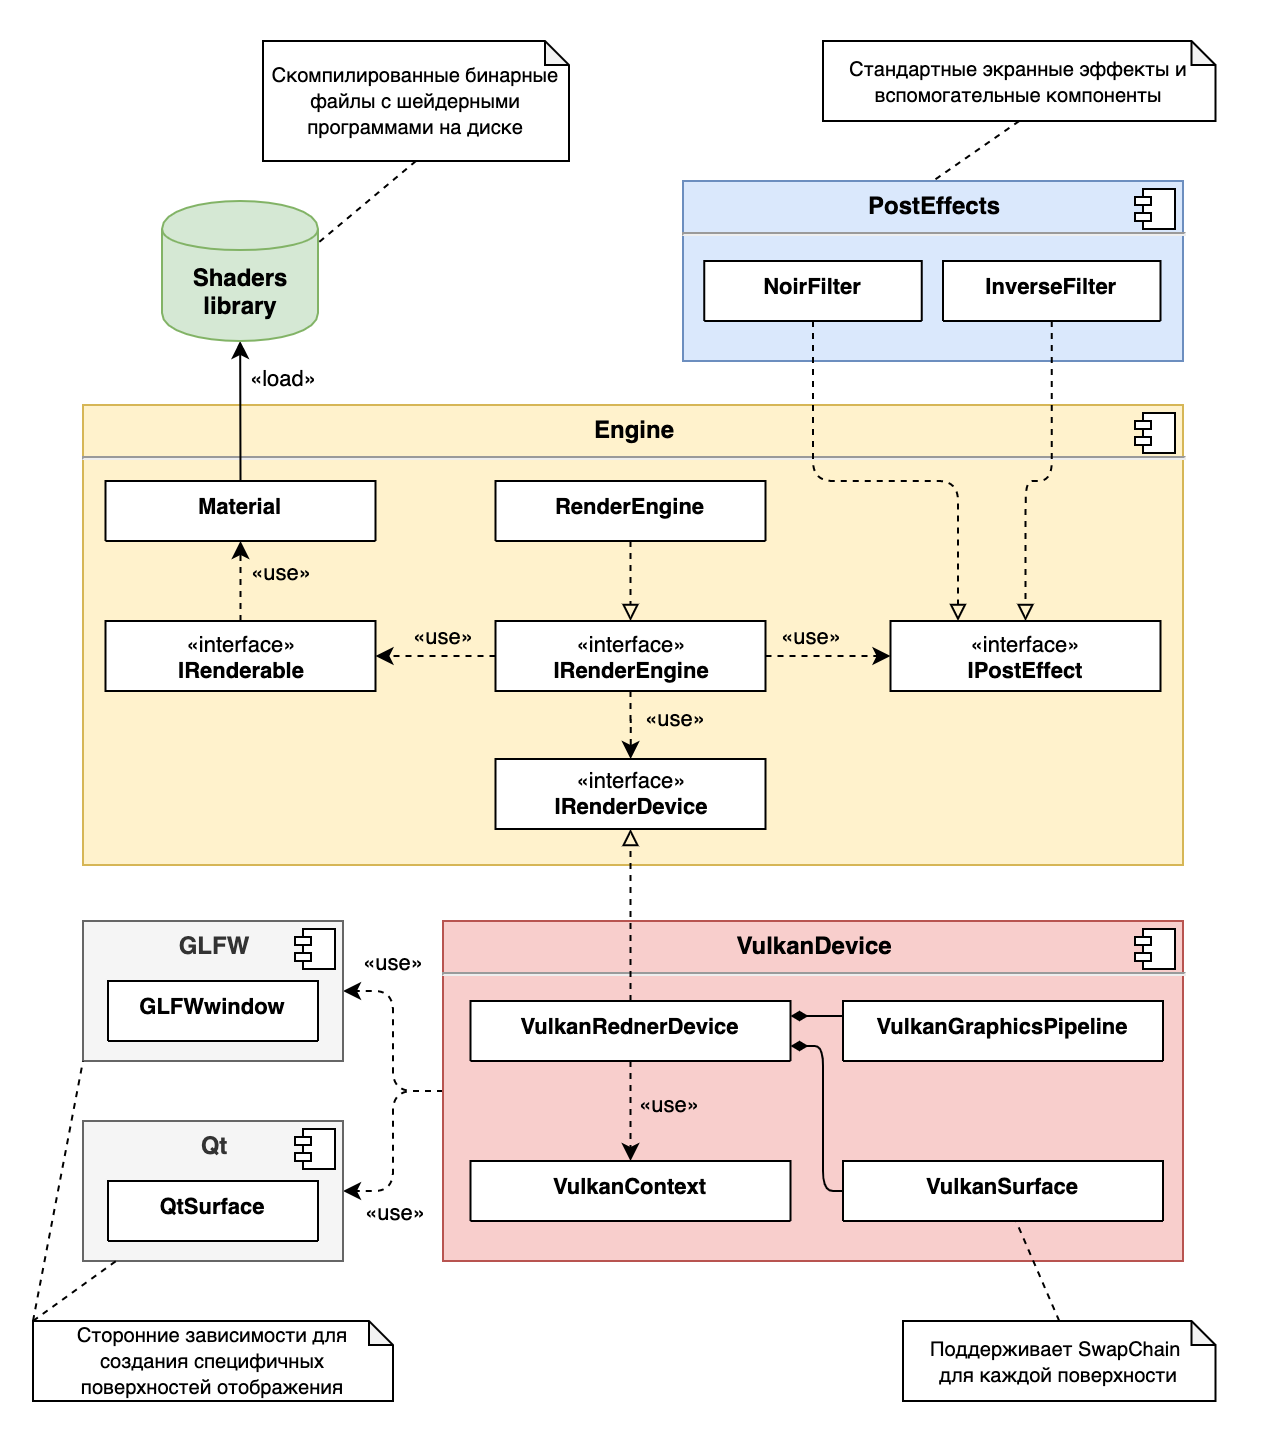
\includegraphics[width=1.0\textwidth]{pictures/IgnimbriteStructure}
     \label{fig:library:uml}
\end{figure}

\subsection{Поддержка Vulkan API}

Для поддержки доступа к GPU с использованием API Vulkan был разработан модуль VulkanDevice, который реализует интерфейс абстрактного графического девайса и полностью инкапсулирует логику взаимодействия с этим API.  

В рамках данной работы были реализованы следующие компоненты модуля VulkanDevice:

\begin{itemize}
    \item \textbf{VulkanContex}: контекст графической библиотеки Vulkan, который инкапсулирует логику инициализации библиотеки, выбора и конфигурации графического девайса, а также расширений, требуемых для создания приложения с использованием Vulkan для конкретной операционной системы. 
    \item \textbf{VulkanSwapchain}: объект, который инкапсулирует логику презентации финального изображения, сгенерированного на GPU, в специфичное окно или поверхность операционной системы. API Vulkan требует осуществлять явную синхронизации CPU и GPU для доступа к изображению, а также выполнять обработку событий изменения поверхности отображения или конфигурацию \textit{режима презентации}~\cite{spec:vulkan} в зависимости от возможностей конечной системы и требований приложения.
    \item \textbf{VulkanGraphicsPipeline}: конвейер растеризации геометрических примитивов с использованием Z-буффера, который включает в себя настройку полностью программируемых этапов, таких как вершинные и фрагментные шейдеры, и частично конфигурируемых --- сборка примитивов, растеризация, тест глубины и трафарета, а также альфа-смешивание. В отличие от графического API OpenGL, который позволяет динамически изменять процесс растеризации без явного создания объектов конфигурации, API Vulkan требует мануального создания полностью сконфигурированного неизменяемого графического конвейера, который позже может быть использован для отображения примитивов.
\end{itemize}

\subsection{Система визуализации}

Для доступа к графической функциональности высокого уровня был реализован класс \textbf{RenderEngine}, который поддерживает список видимых объектов и источников света на сцене, а также осуществляет отображения этих объектов в окно операционной системы или внеэкранный буфер.

Видимые объекты сцены реализуют интерфейс \textbf{IRenderable}, что позволяет им реагировать на события, генерируемые RenderEngine, и отображать себя независимо от структуры сцены или окружения. В качестве стандартной реализации представлен \textbf{RenderableMesh}, который позволяет отображать геометрию, состоящую из индексированных вершин с фиксированным числом атрибутов.

Для конфигурации отображения реализован \textbf{Material}, который хранит состояние конвейера растеризации, а также поддерживает произвольные параметры отображения, которые могут быть установлены посредством типобезопасного интерфейса, автоматически упакованы и скопированы в видеопамять для последующего использования при отображении на GPU. Материалы поддерживают раздельное владение ресурсами GPU, что позволяет сократить расход видеопамяти и уменьшить число изменений состояния GPU за счет предварительно упорядочивания отображаемых объектов в зависимости от их материалов.  

В качестве стандартных алгоритмов освещения доступны:

\begin{itemize}
    \item Затенение объекта выбранным фиксированным цветом
    \item Затенение объекта с учетом интенсивности освещения сцены на основе модели Ламберта с использованием теневых карт для создания теней
    \item Физически-корректное затенение с учетом интенсивности освещения на основе вариации модели Кука-Торренса, которая была предложена в работе Брайана Кариса~\cite{pbr:unreal:engine} как одна из наиболее визуально приемлемых моделей для вычисления в режиме реального времени. На рис.~\ref{fig:helmet:pbr} представлен пример отображения геометрии с использованием данного алгоритма затенения.
\end{itemize}

\begin{figure}[]
     \caption{Физически-корректное затенение 3D-геометрии с использованием вариации модели
     Кука-Торренса}
     \centering
     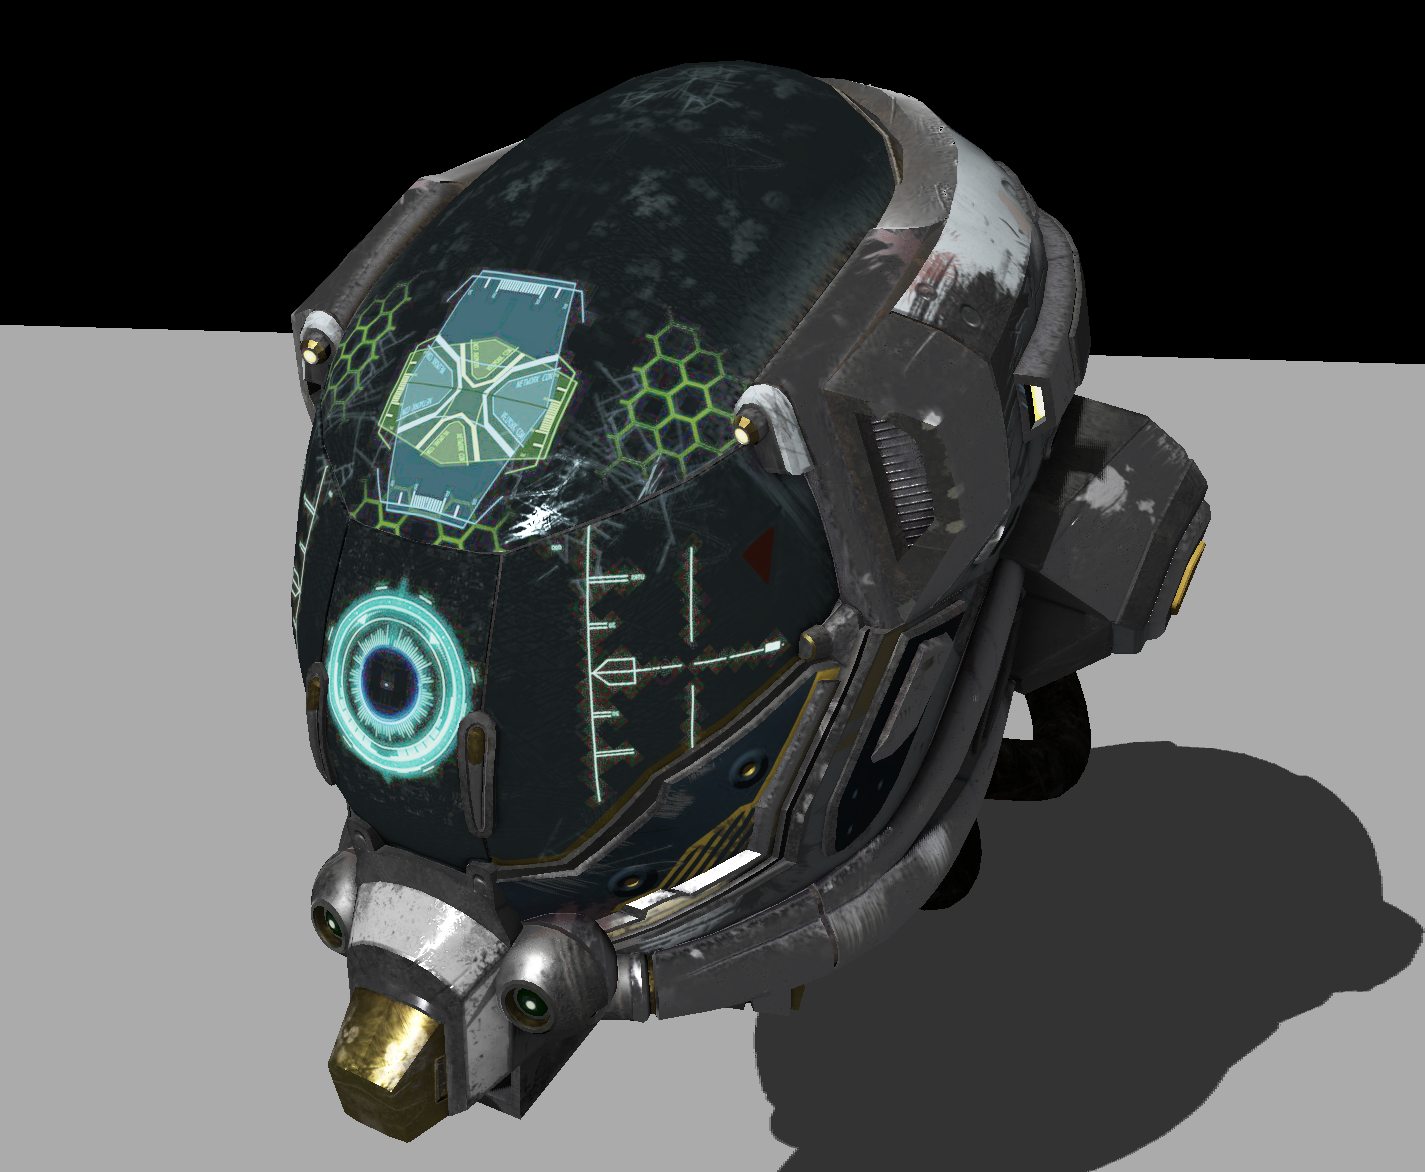
\includegraphics[width=0.9\textwidth]{pictures/Helmet}
     \label{fig:helmet:pbr}
\end{figure}

Объекты, реализующие интерфейс \textbf{IPostEffect}, позволяют последовательно применять экранные эффекты к сформированному в процессе растеризации изображению. Для каждого эффекта доступна информация о цвете точки и ее глубине в соответствующем Z-буфере. В качестве стандартных эффектов реализованы черно-белый фильтр и фильтр инвертирования цвета, пример применения которых представлен на рис.~\ref{fig:effects}. 

\begin{figure}[]
     \caption{Применение экранных эффектов к растеризованному изображению}
     \centering
     \begin{subfigure}[b]{0.44\textwidth}
        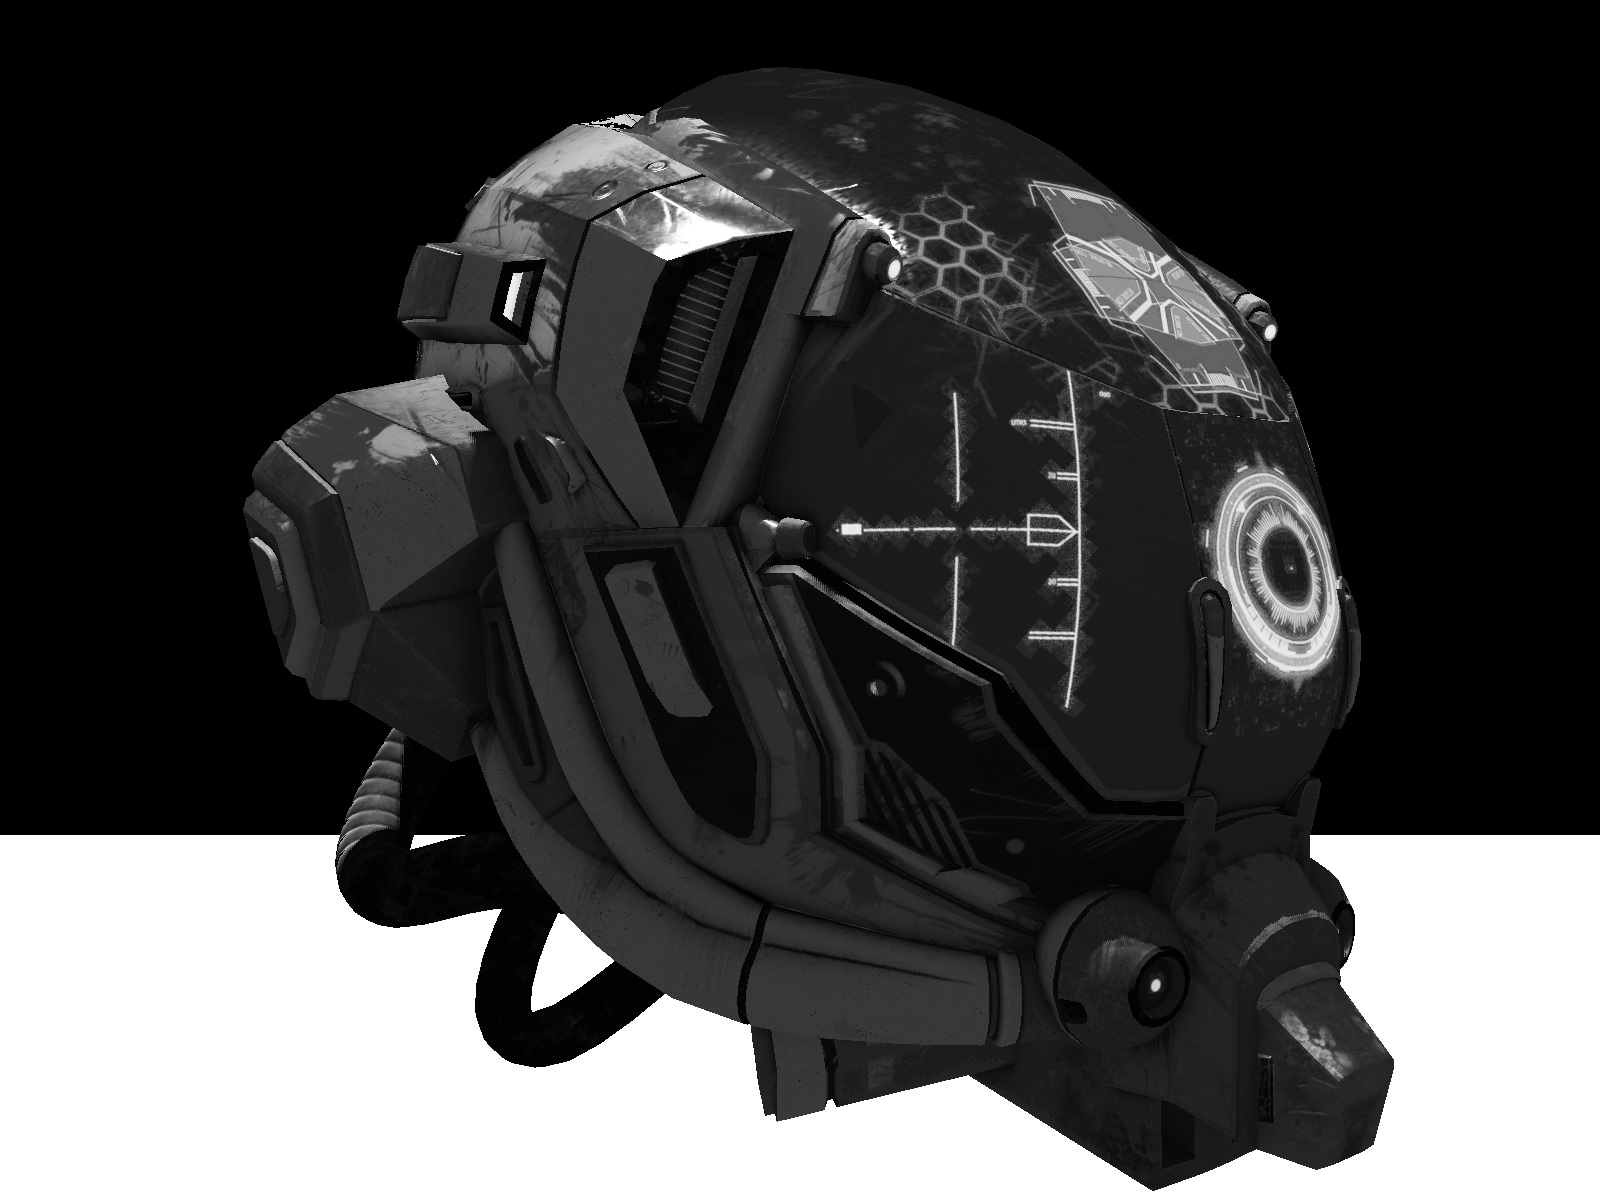
\includegraphics[width=\textwidth]{pictures/Noir}
        \caption{Черно-белый фильтр}
        \label{fig:effects:white:black}
    \end{subfigure}
    ~
    \begin{subfigure}[b]{0.44\textwidth}
        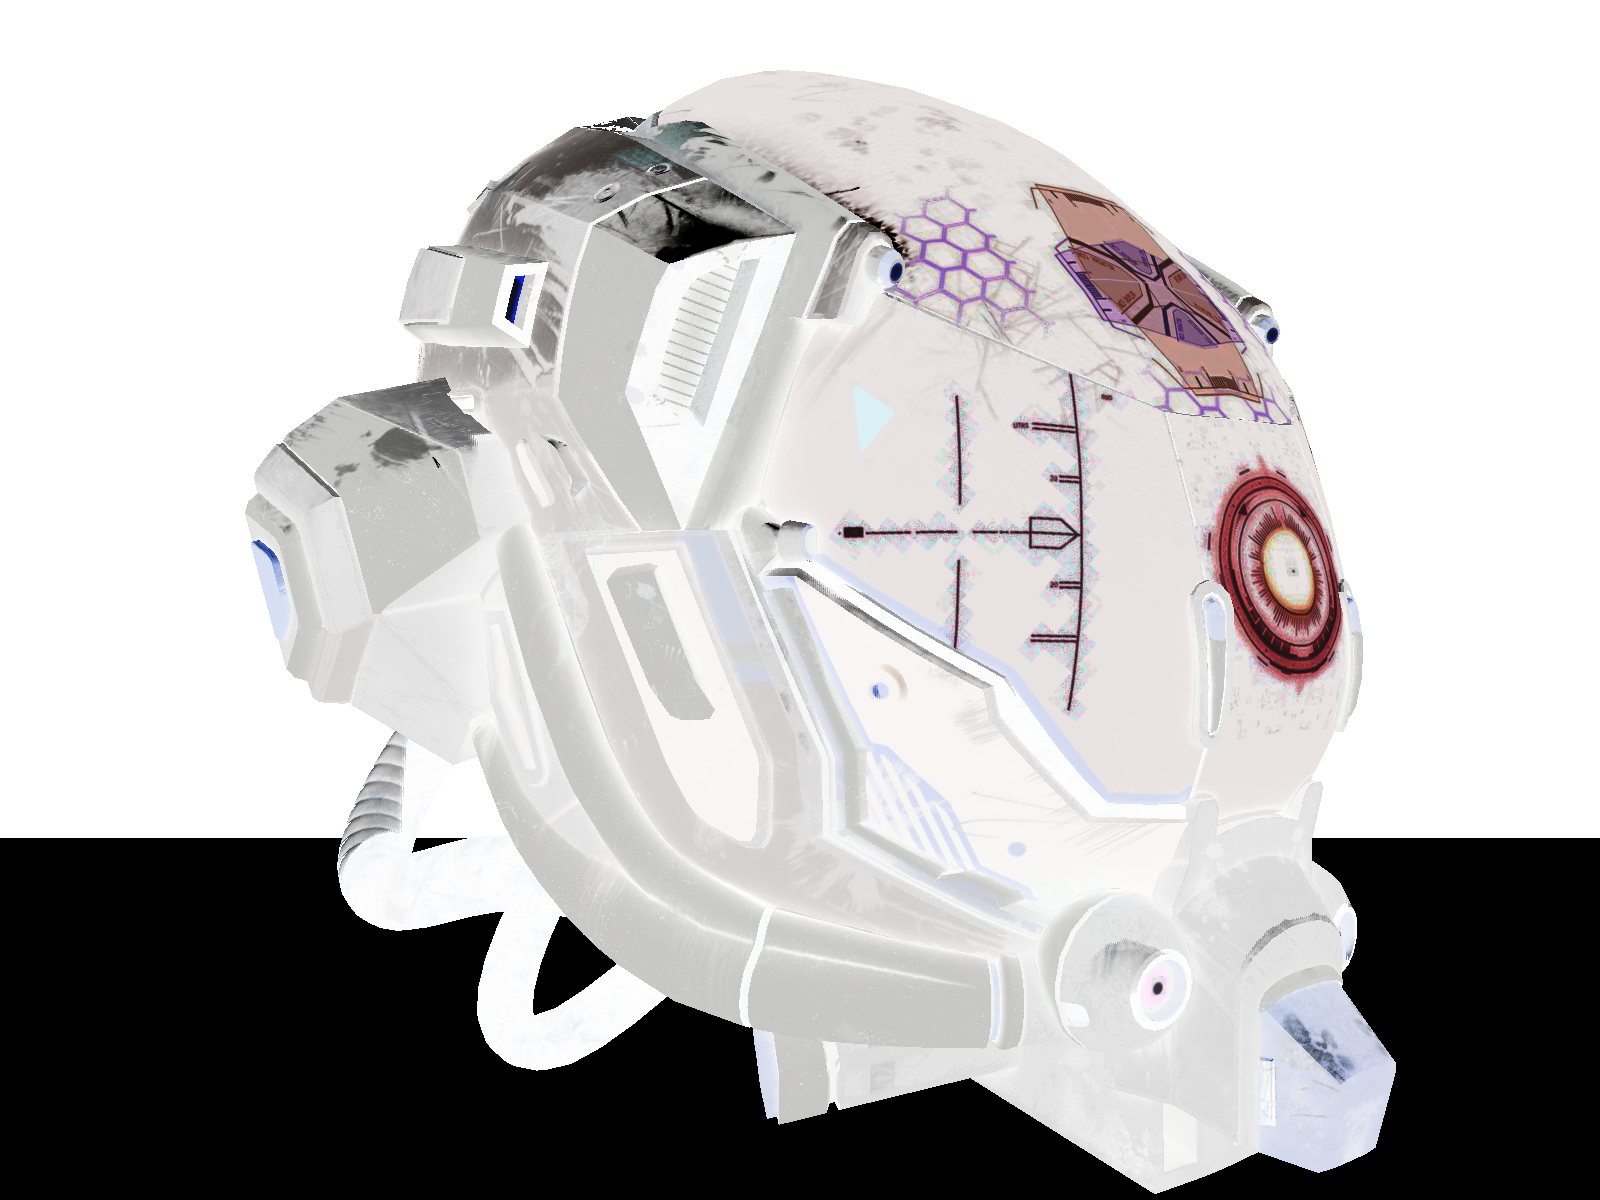
\includegraphics[width=\textwidth]{pictures/Inverse}
        \caption{Фильтр инвертирования цвета}
        \label{fig:effects:inverse}
    \end{subfigure}
    
    \label{fig:effects}
\end{figure}

% ---------------------------------------------------------------------------- %

\section*{Заключение}

В ходе выполнения работы получены следующие результаты:

\begin{itemize}
    \item Проведено исследование предметной области
    \item Проведено сравнение существующих решений
    \item Разработаны и формализованы требования к проекту
    \item Реализованы компоненты библиотеки в соответствии с заявленными требованиями
    \item Реализована поддержка Vulkan API
\end{itemize}

Реализованная графическая библиотека была успешно \textit{интегрирована} в проект CoreCVS студентом 371 группы Сультимом Цырендашиевым в рамках его курсовой работы. В качестве основы для интеграции использовалась платформа Qt виджетов для создания поверхности отображения. 

Несмотря на скромную функциональность реализованной графической библиотеки, ее ядро в сочетании с поддержкой Vulkan API будет использовано в дальнейшем для расширения и создания 3D визуализации уже в рамках проекта CoreCVS.

% ---------------------------------------------------------------------------- %

\setmonofont[Mapping=tex-text]{CMU Typewriter Text}
\bibliographystyle{ugost2008ls}
\bibliography{3d_graphics_vulkan.bib}
\end{document}
